\documentclass[aspectratio=169]{../latex_main/tntbeamer}  % you can pass all options of the beamer class, e.g., 'handout' or 'aspectratio=43'
\usepackage{dsfont}
\usepackage{bm}
\usepackage[english]{babel}
\usepackage[T1]{fontenc}
%\usepackage[utf8]{inputenc}
\usepackage{graphicx}
\graphicspath{ {./figures/} }
\usepackage{algorithm}
\usepackage[ruled,vlined,algo2e,linesnumbered]{algorithm2e}
\usepackage{hyperref}
\usepackage{booktabs}
\usepackage{mathtools}

\usepackage{amsmath,amssymb}

\DeclareMathOperator*{\argmax}{arg\,max}
\DeclareMathOperator*{\argmin}{arg\,min}

\usepackage{amsbsy}
\newcommand{\vect}[1]{\bm{#1}}
%\newcommand{\vect}[1]{\boldsymbol{#1}}

\usepackage{pgfplots}
\pgfplotsset{compat=1.16}
\usepackage{tikz}
\usetikzlibrary{trees} 
\usetikzlibrary{shapes.geometric}
\usetikzlibrary{positioning,shapes,shadows,arrows,calc,mindmap}
\usetikzlibrary{positioning,fadings,through}
\usetikzlibrary{decorations.pathreplacing}
\usetikzlibrary{intersections}
\pgfdeclarelayer{background}
\pgfdeclarelayer{foreground}
\pgfsetlayers{background,main,foreground}
\tikzstyle{activity}=[rectangle, draw=black, rounded corners, text centered, text width=8em]
\tikzstyle{data}=[rectangle, draw=black, text centered, text width=8em]
\tikzstyle{myarrow}=[->, thick, draw=black]

% Define the layers to draw the diagram
\pgfdeclarelayer{background}
\pgfdeclarelayer{foreground}
\pgfsetlayers{background,main,foreground}

% Requires XeLaTeX or LuaLaTeX
%\usepackage{unicode-math}

\usepackage{fontspec}
%\setsansfont{Arial}
\setsansfont{RotisSansSerifStd}[ 
Path=../latex_main/fonts/,
Extension = .otf,
UprightFont = *-Regular,  % or *-Light
BoldFont = *-ExtraBold,  % or *-Bold
ItalicFont = *-Italic
]
\setmonofont{Cascadia Mono}[
Scale=0.8
]

% scale factor adapted; mathrm font added (Benjamin Spitschan @TNT, 2021-06-01)
%\setmathfont[Scale=1.05]{Libertinus Math}
%\setmathrm[Scale=1.05]{Libertinus Math}

% other available math fonts are (not exhaustive)
% Latin Modern Math
% XITS Math
% Libertinus Math
% Asana Math
% Fira Math
% TeX Gyre Pagella Math
% TeX Gyre Bonum Math
% TeX Gyre Schola Math
% TeX Gyre Termes Math

% Literature References
\newcommand{\lit}[2]{\href{#2}{\footnotesize\color{black!60}[#1]}}

%%% Beamer Customization
%----------------------------------------------------------------------
% (Don't) Show sections in frame header. Options: 'sections', 'sections light', empty
\setbeamertemplate{headline}{empty}

% Add header logo for normal frames
\setheaderimage{
	% 
\includegraphics[height=\logoheight]{figures/TNT_darkv4.pdf}
	
\includegraphics[height=\logoheight]{../latex_main/figures/luh_logo_rgb_0_80_155.pdf}
	% 
\includegraphics[height=\logoheight]{figures/logo_tntluh.pdf}
}

% Header logo for title page
\settitleheaderimage{
	% 
\includegraphics[height=\logoheight]{figures/TNT_darkv4.pdf}
	
\includegraphics[height=\logoheight]{../latex_main/figures/luh_logo_rgb_0_80_155.pdf}
	% 
\includegraphics[height=\logoheight]{figures/logo_tntluh.pdf}
}

% Title page: tntdefault 
\setbeamertemplate{title page}[tntdefault]  % or luhstyle
% Add optional title image here
%\addtitlepageimagedefault{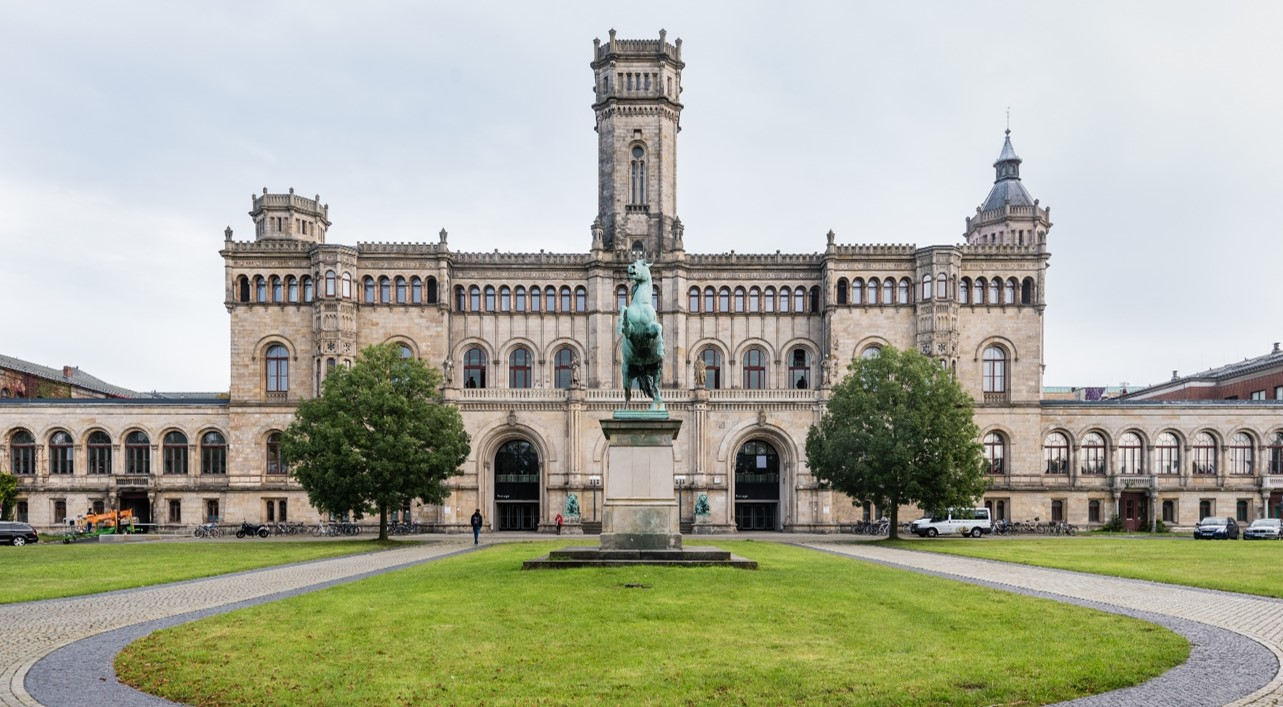
\includegraphics[width=0.65\textwidth]{figures/luh_default_presentation_title_image.jpg}}

% Title page: luhstyle
% \setbeamertemplate{title page}[luhstyle]
% % Add optional title image here
% \addtitlepageimage{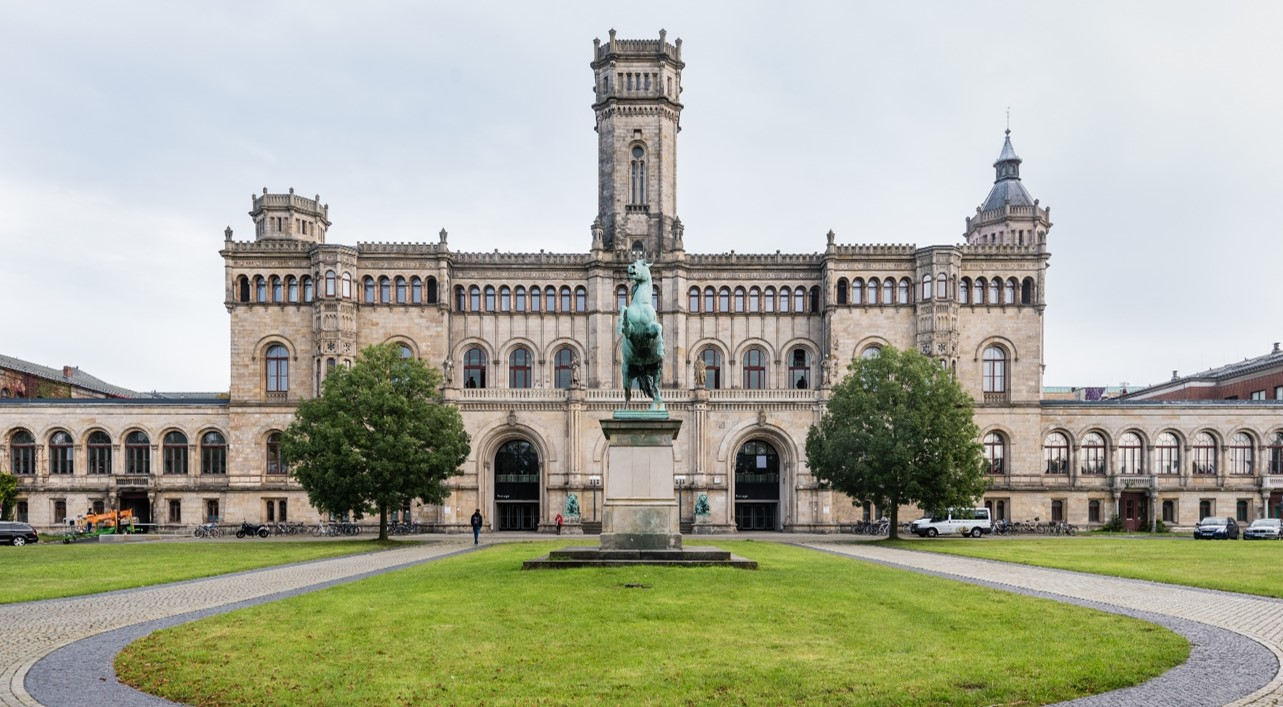
\includegraphics[width=0.75\textwidth]{figures/luh_default_presentation_title_image.jpg}}

\author[Abedjan \& Lindauer]{Ziawasch Abedjan \& Marius Lindauer\\[1em]
	
\includegraphics[height=\logoheight]{../latex_main/figures/luh_logo_rgb_0_80_155.pdf}\qquad
	
\includegraphics[height=\logoheight]{../latex_main/figures/DBIS_Kurzlogo.png}\qquad

\includegraphics[height=\logoheight]{../latex_main/figures/TNT_darkv4}\qquad

\includegraphics[height=\logoheight]{../latex_main/figures/L3S.jpg}	}
\date{Summer Term 2022; \hspace{0.5em} {
\includegraphics[height=1.5em]{../latex_main/figures/Cc-by-nc-sa_icon.svg.png}}; based on \href{https://ds100.org/fa21/}{[DS100]}
}


%%% Custom Packages
%----------------------------------------------------------------------
% Create dummy content
\usepackage{blindtext}

% Adds a frame with the current page layout. Just call \layout inside of a frame.
\usepackage{layout}


%%% Macros
%\renewcommand{\vec}[1]{\mathbf{#1}}
% \usepackage{bm}
%\let\vecb\bm

\title[Introduction]{DS: Gradient Descent}
\subtitle{Optimizing Loss in 1D}

\graphicspath{ {./figure/} }
%\institute{}


\begin{document}
	
	\maketitle
	\begin{frame}{Optimization Goal}
	    Suppose we want to create a model that predicts the tip given the total bill for a table at a restaurant.\\
	    \bigskip
	    \begin{columns}
	     \begin{column}{.5\textwidth}
	        \\
	         For this problem, we’ll keep things simple and have only 1 parameter: gamma.
	             \begin{equation*}
	                 \hat{y}  = f_{\hat{\gamma}}(\Vec{x})  = \hat{\gamma}\Vec{x}
                \end{equation*}
	            \begin{itemize}
                     \item In other words, we are fitting a line with zero y-intercept.
	             \end{itemize}
	             \bigskip
	             See Notebook.
	     \end{column}
	     
	     
	     \begin{column}{.5\textwidth}
	        %\vspace{-2.5cm}
	            \\
              \hspace{0cm} 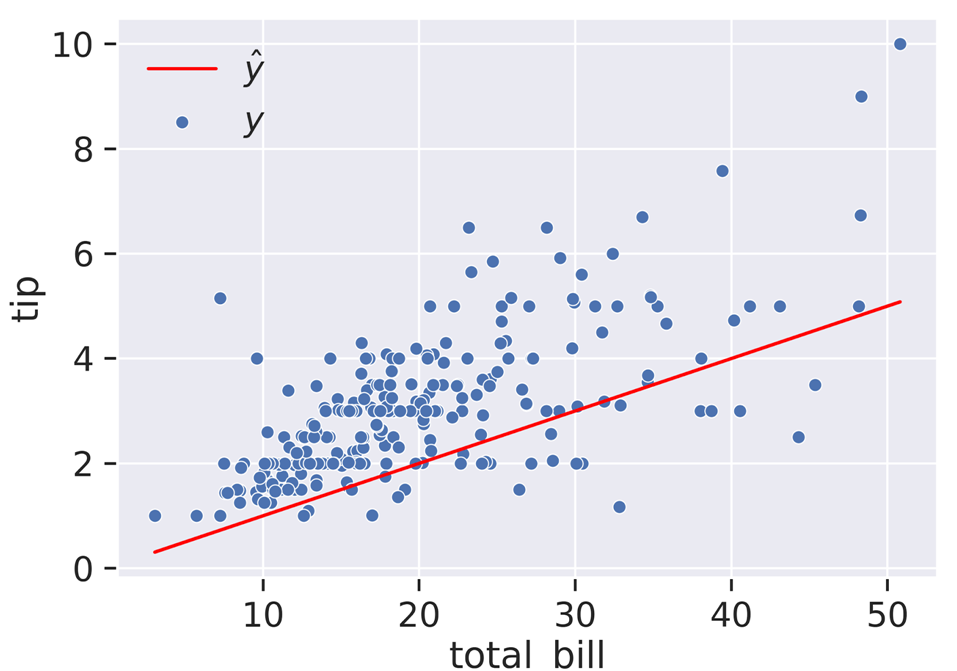
\includegraphics[scale=.4]{Bild9}\\
	         %\vspace{2.5cm}
	     \end{column}
	    \end{columns}
	\end{frame}
	
	
	
	\begin{frame}[c]{Optimization Goal}
	    As discussed before, picking the best gamma is meaningless unless we pick:
	    \begin{itemize}
	        \item Loss function.
	        \item Regularization term.
	    \end{itemize}
	    For this example, let’s use the L2 loss and no regularization.
	\end{frame}
	
	
	
	\begin{frame}{Solution Approach \#1: Closed Form Solution}
	    One approach is to use a closed form solution. 
	    \begin{itemize}
	        \item On HW5 problem 3, you derived the closed form expression below:
	        \begin{equation*}
	            \hat{\gamma} = \frac{\sum x_iy_i}{\sum x_i^2}
	        \end{equation*}
	        Another closed form expression is just our standard normal equation:
	        \begin{equation*}
	            \hat{\gamma} = (\mathbb{X}^T\mathbb{X})^{-1}\mathbb{X}^T\Vec{y}
	        \end{equation*}
	    \end{itemize}
	\end{frame}
	
	\begin{frame}{Solution Approach \#2A: Brute Force Plotting}
	    Another approach is to plot the loss and eyeball the minimum.\\
	    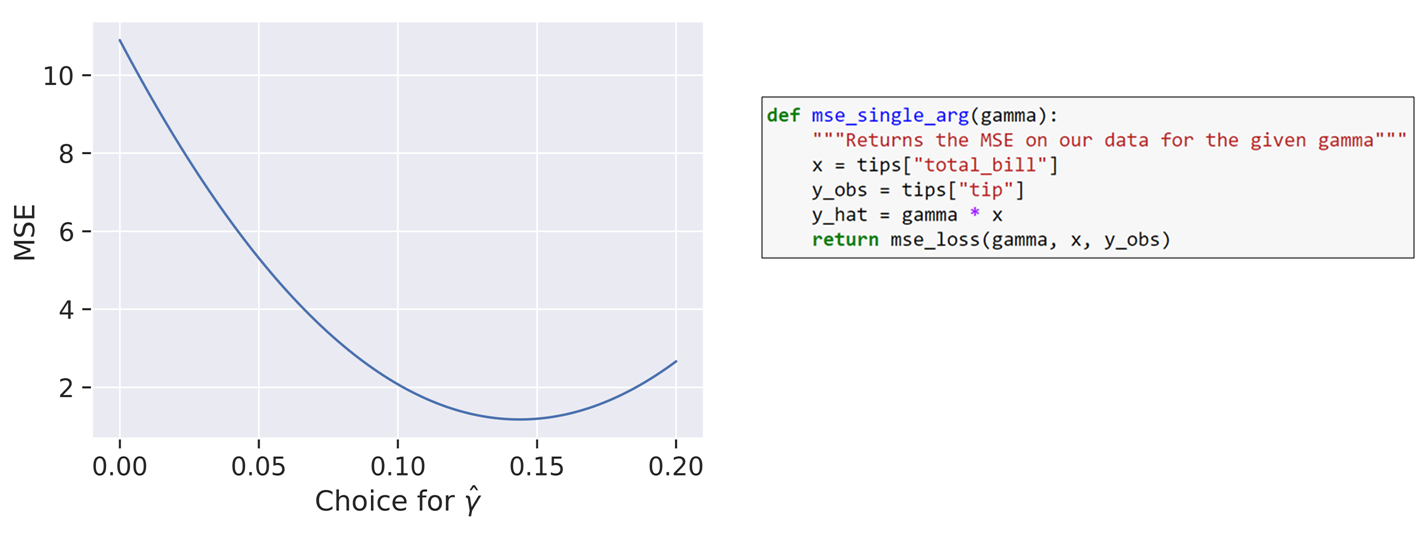
\includegraphics[scale=.4]{Bild10}
	\end{frame}
	
	
	\begin{frame}{Solution Approach #2B: Brute Force}
	    A related approach: Try a bunch of gammas and simply keep the best one.\\
	    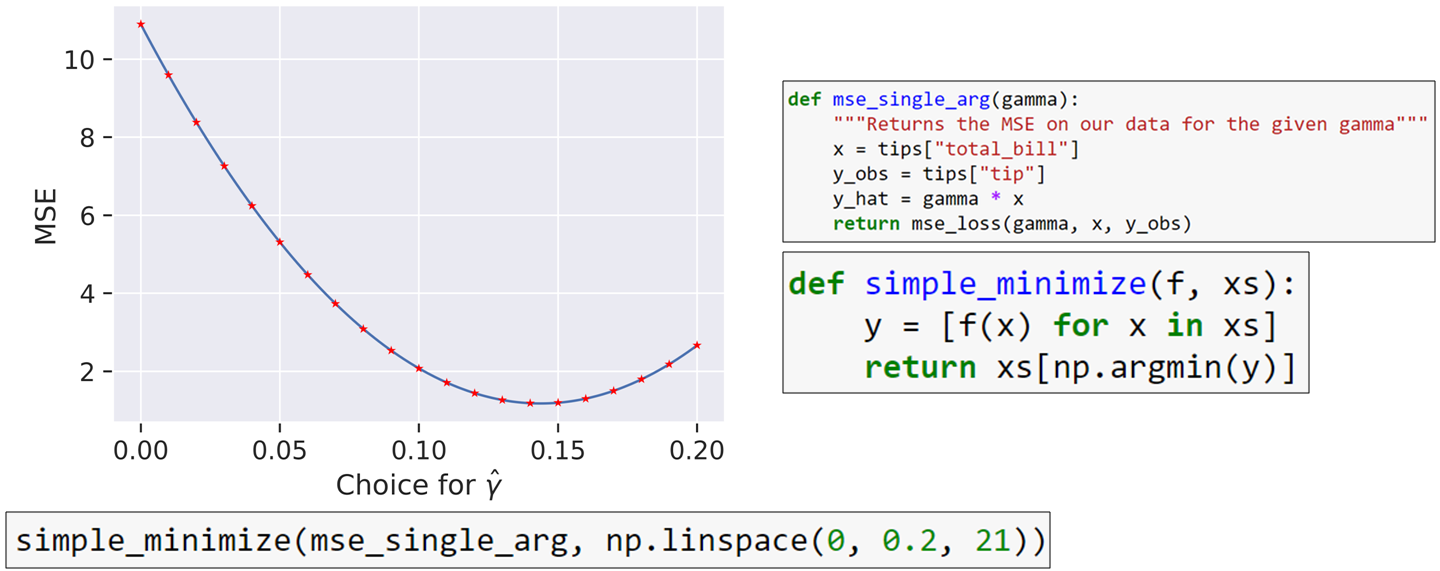
\includegraphics[scale=.4]{Bild11}
	\end{frame}
	
	
	\begin{frame}{Solution Approach #3: Use Gradient Descent}
	    We can use our gradient descent algorithm from before.
	    \begin{itemize}
	        \item To use this, we need to find the derivative of the function that we’re trying to minimize.
	        \item Earlier, we minimized an arbitrary 4th degree polynomial.
	    \end{itemize}
	    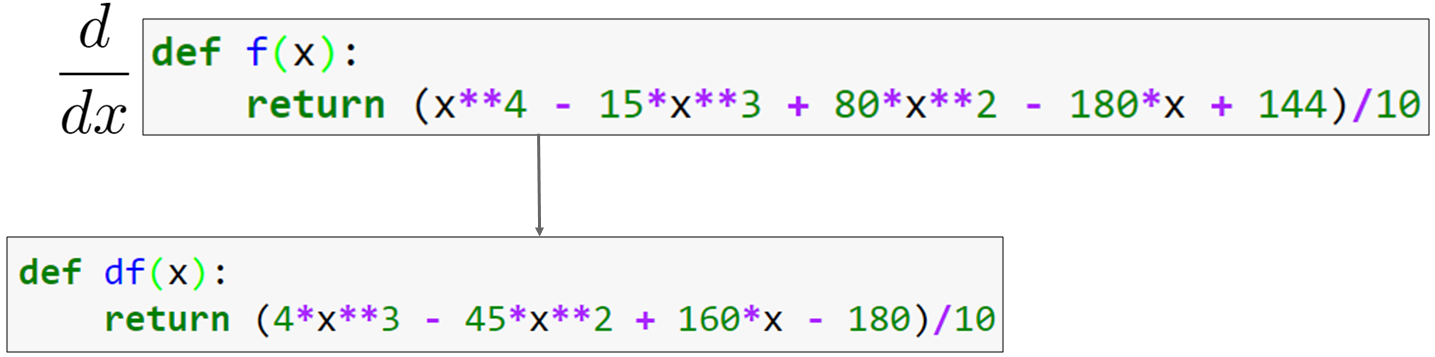
\includegraphics[scale=.4]{Bild12}
	\end{frame}
	
	
	
	\begin{frame}{Solution Approach #3: Use Gradient Descent}
	    We can use our gradient descent algorithm from before.
	    \begin{itemize}
	        \item To use this, we need to find the derivative of the function that we’re trying to minimize.
	        \item Earlier, we minimized an arbitrary 4th degree polynomial.
	    \end{itemize}
	    \centering
	    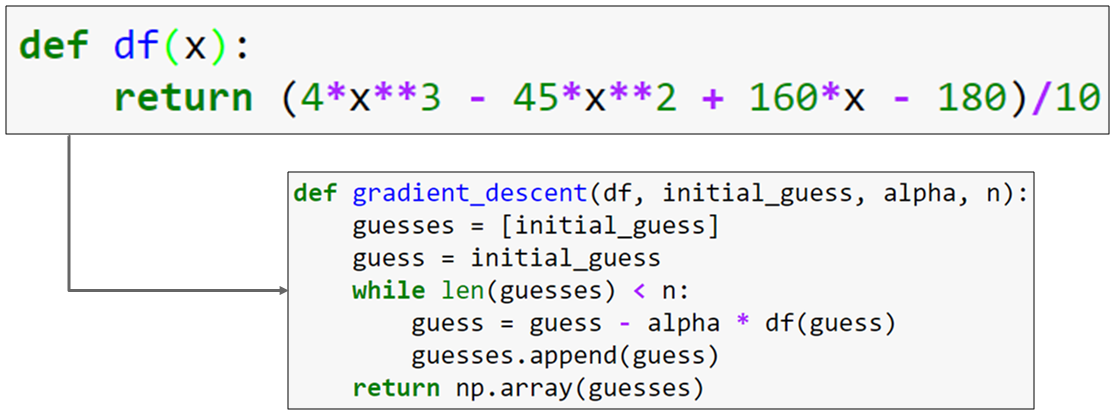
\includegraphics[scale=.4]{Bild13}
	\end{frame}
	
	
	
	\begin{frame}{Solution Approach #3: Use Gradient Descent}
	    We can use our gradient descent algorithm from before.
	    \begin{itemize}
	        \item To use GD on our linear regression problem, we need to find the derivative of the function that we’re trying to minimize, namely mse\_loss.
	    \end{itemize}
	    \centering
	    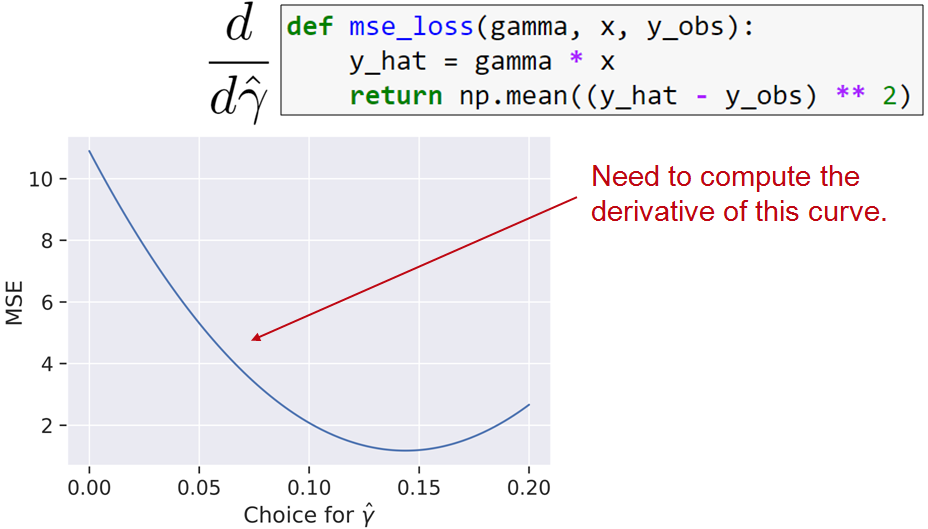
\includegraphics[scale=.35]{Bild14}
	\end{frame}
	
	
	
	\begin{frame}{Solution Approach #3: Use Gradient Descent}
	    We can use our gradient descent algorithm from before.
	    \begin{itemize}
	        \item To use GD on our linear regression problem, we need to find the derivative of the function that we’re trying to minimize, namely mse\_loss.
	    \end{itemize}
	    \centering
	    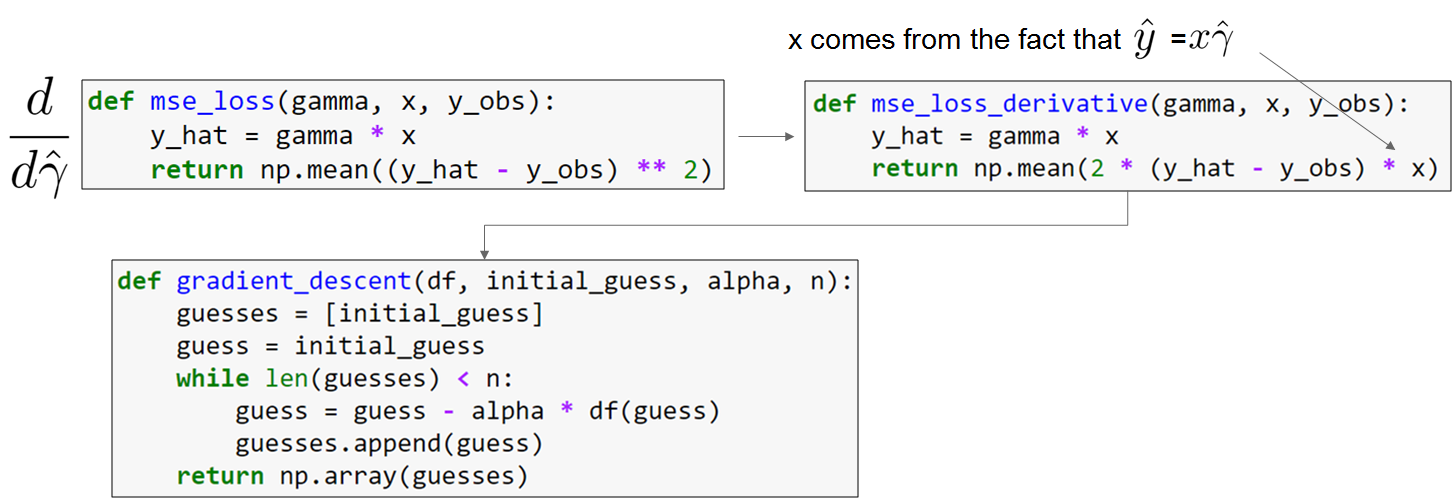
\includegraphics[scale=.38]{Bild15}
	\end{frame}
	
	
	
	\begin{frame}[c]{Solutions \#4/\#5: scipy.optimize.minimize / scipy.linear\_model}
	    As before, we can also use the scipy.optimize.minimize or scipy.linear\_model libraries. Because it’s exactly the same as before, we omit the exact details from this lecture.\\
	    \bigskip
	    Ultimately, both of these approaches use a numerical method similar to gradient descent.
	\end{frame}
\end{document}